\chapter{Opis projektnog zadatka}
		\textbf{\textit{dio 1. revizije}}\\
		
		\textit{Na osnovi projektnog zadatka detaljno opisati korisničke zahtjeve. Što jasnije opisati cilj projektnog zadatka, razraditi problematiku zadatka, dodati nove aspekte problema i potencijalnih rješenja. Očekuje se minimalno 3, a poželjno 4-5 stranica opisa.	Teme koje treba dodatno razraditi u ovom poglavlju su:}
			%\textit{potencijalna korist ovog projekta}
			\par
			Cilj je razviti programsku potporu za web aplikaciju \textit{"MapTasker"} koja služi za pronalaženje nestalih osoba tijekom raznim elementarnih nepogoda. Kako bi se takve operacije uspješno izvele, potrebno je spasiocima napraviti kartu s pozicijama kuća koju proizvode kartografi. Područje koje je potrebno kartografirati postavljaju voditelji.
			
			Početna stranica sadrži formu za registraciju ili prijavu te tipku za prijavu nestalih osoba. Taj gumb vodi korisnika na stranicu na kojoj se nalaze već prijavljene nestale osobe te gumb za prijavu nove osobe. Prijavljenim korisnicima se na stranici također nalazi karta čije se funkcionalnosti razlikuju, oviseći o ulozi korisnika. Uz kartu se nalazi statistika koja voditeljima i kartografima prikazuje podatke o nestalim i pronađenim osobama, broj završenih blokova kroz vrijeme (\textit{engl. Burn down chart}) te broj pretraženih i nepretraženih građevina.
			
			Prijavljeni korisnici imaju pristup stranici koja im omogućuje pregled i uređivanje njihovog profila.
			Pri pokretanju aplikacije neregistrirani korisnik ima dvije opcije:
			\begin{enumerate}
				\item Ostati neregistriran te prijaviti nestalu osobu te njihove informacije:
				\begin{itemize}
					\item Ime i prezime
					\item Fotograija
					\item Opis nestale osobe
				\end{itemize}
				\item Poslati zahtjev za registraciju na aplikaciju pri čemu je potrebno navesti:
				\begin{itemize}
					\item Uloga za koju se prijavljuje (spasioc, voditelj, kartograf)
					\item Korisničko ime
					\item Fotografija
					\item Lozinka
					\item Ime i prezime
					\item Broj mobitela
					\item Email adresa
				\end{itemize}
			\end{enumerate}
			
			U prvom slučaju gdje korisnik prijavljuje nestalu osobu, ostali korisnici mogu komentirati prijavu i odgovoriti na nju. Kad je prijavljena osoba pronađena, spasioc ili voditelj zaključavaju prijavu dok voditelj jedini ima ulogu brisanja prijave i komentara.
			
			\underbar{Voditelj} je odgovoran za proces stvaranja operacije te definiranja područja koje će se kartografirati i pretraživati. To uključuje određivanje područja na karti koje će biti definirano poligonom. Kako bi se izbjegli problemi, samo jedan voditelj može raditi na jednoj regiji i blokovima.
			Postoje tri razine područja:
			\begin{itemize}
				\item Regija
				\item Blok
				\item Građevina
			\end{itemize}
			
			Na jednom poligonu može postojati više regija u kojima se nalaze razni blokovi. Svaki od blokoba ima status o tome u kojoj se fazi trenutno nalazi:
			\begin{enumerate}
				\item \textbf{Nezapočeto}
				\item \textbf{Aktivno}
				\item \textbf{Provjera}
				\item \textbf{Završeno}
			\end{enumerate}
			
			Blok će biti prikazan na karti u različitim bojama ovisno o fazi. Nakon što je blok \textbf{završen}, voditelj zaključava operaciju.
			
			\underbar{Kartograf} jedini može mijenjati statuse blokova iz \textbf{nezapočetog} u \textbf{aktivnog} i nakon toga u \textbf{provjeru}. U fazu \textbf{završeno} blok prelazi jedino kad su dva kartografa sigurna da je posao dobro obavljen. Ako kartograf smatra da se posao mogao bolje odraditi, može vratiti stanje bloka iz \textbf{provjere} u \textbf{aktivno}. U \textbf{aktivnom} stanju kartograf može dodavati nove građevine. Kartograf može tijekom kartografiranja imati samo jedan \textbf{aktivan} blok kako bi se izbjegli konflikti. Blok može biti \textbf{aktivan} samo kod jednog kartografa.
			
			\underline{Spasioc} na svojoj stranici ima pristup karti s građevinama koje imaju jedan od dva statusa:
			\begin{itemize}
				\item Pretraženo
				\item Nepretraženo
			\end{itemize}
			
			Nakon promjene statusa iz \textbf{nepretraženo} u \textbf{pretraženo}, kartograf i voditelj primaju obavijest na stranici da je osoba za koju je objavljena prijava pronađena te voditelj dobiva ime i prezime spasioca. U tom slučaju, voditelj zatvara prijavu za pronađenu osobu. Time se ažurira statistika \textit{Burn down chart}, broj nestalih osoba i pretraženih građevina. 
			
			\underline{Administrator} aplikacije ima pristup popisu svih registriranih korisnika te njihovim osobnim podatcima. Uloga mu je potvrđivanje ili odbacivanje zahtjeva za registraciju korisnika te može mijenjati dodijeljena prava korisnicima.
			

            Na internetu već je dostupna aplikacija slična \textit{MapTaskeru} po imenu \textbf{Međunarodne komisije za nestale osobe} (\textit{International Commission on Missing Persons}). Prijave nestalih osoba preko \textit{MapTaskera} i \textit{ICMP-a} postoje mnoge sličnosti i razlike. 

            \underline{\textbf{Sličnosti:}} Informacije koje je potrebno popuniti tijekom prijave, kao što su ime, prezime te opis nestale osobe. Moguće je dodati fotografiju osobe koja će postati vidljiva javnosti te njezini članovi mogu komentirati jesu li vidjeli nestalu osobu.

            \underline{\textbf{Razlike:}} U formi za prijavu su dostupna dodatna polja za popunjavanje: spol, datum rođenja, država i grad kojoj osoba pripada, datum i mjesto nestanka osobe, visina i težina. Preko ICMP-a anonimna prijava nestale osobe nije moguća pošto je obavezno popuniti i polja s podatcima osobe koja stvara prijavu. Također je moguće poslati liste ili baze podataka koje sadrže informacije o nestalim osobama.


            \underline{\textbf{Moguća proširenja}} bi uključivala dodatna polja informacije o nestaloj osobi kao što su mjerenja, spol te gdje i kada je zadnji put osoba viđena.

            \begin{figure}[H]
			         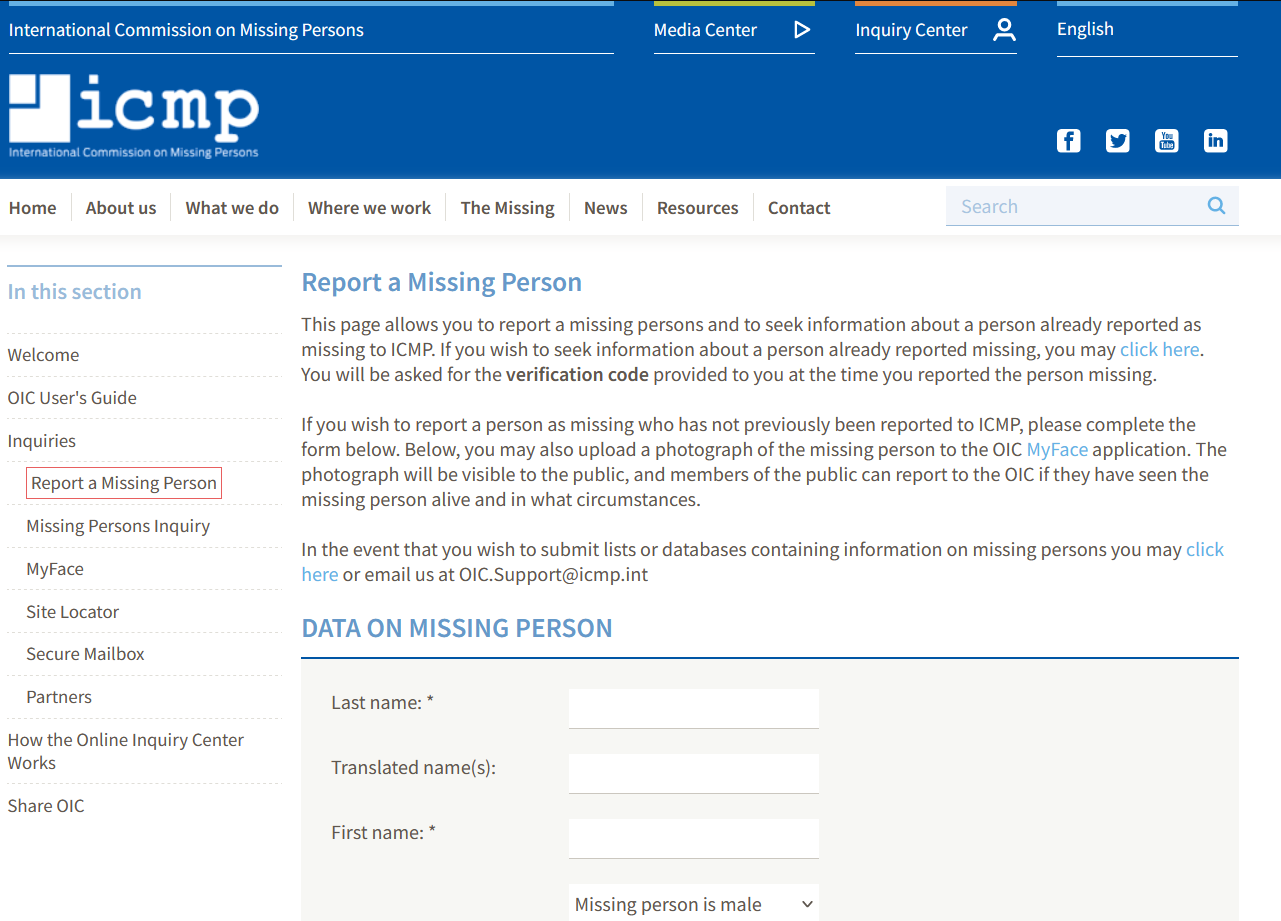
\includegraphics[scale=0.5]{slike/ICMP.png} %veličina slike u odnosu na originalnu datoteku i pozicija slike
			         \centering
			         \caption{Prijava nestale osobe preko ICMP}
			         \label{fig:promjene}
		      \end{figure}


            \begin{figure}[H]
			         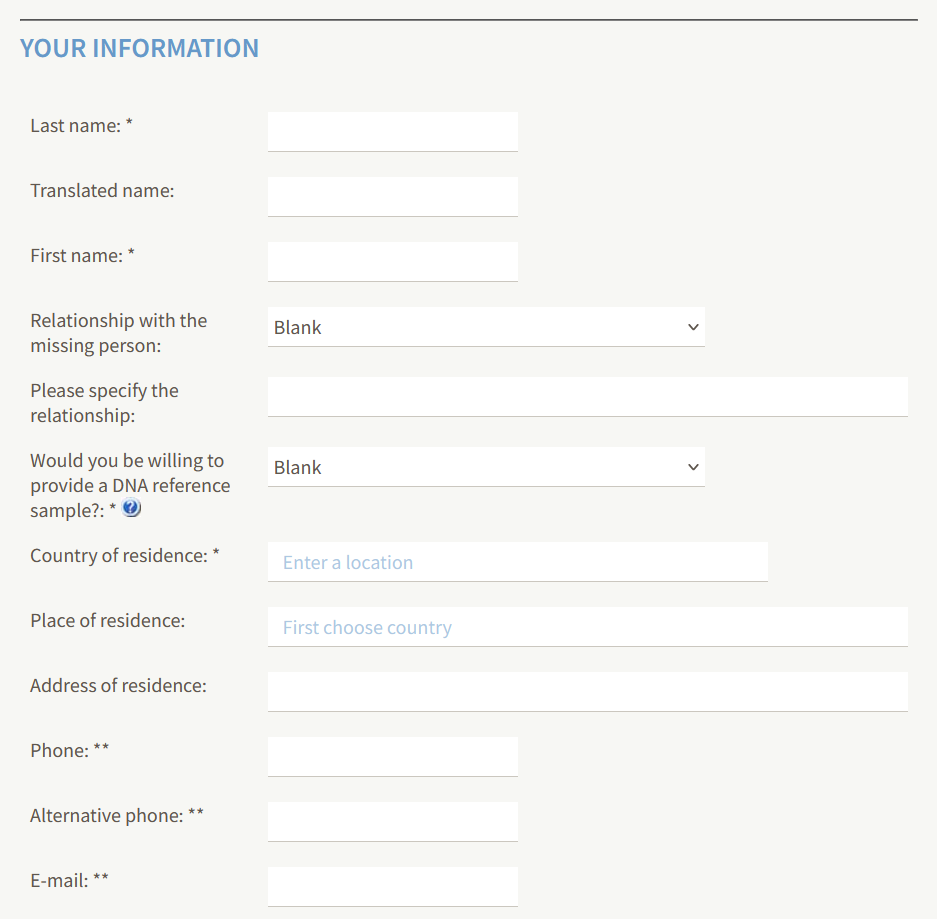
\includegraphics[scale=0.5]{slike/ICMP_2.png} %veličina slike u odnosu na originalnu datoteku i pozicija slike
			         \centering
			         \caption{Popunjavanje informacije korisnika}
			         \label{fig:promjene}
		      \end{figure}


            
			

            
			%\textit{mogućnost prilagodbe rješenja }
			%\textit{opseg projektnog zadatka}
			%\textit{moguće nadogradnje projektnog zadatka}
		
		%\textit{Za pomoć pogledati reference navedene u poglavlju „Popis literature“, a po potrebi konzultirati sadržaj na internetu koji nudi dobre smjernice u tom pogledu.}
		\eject
		
		\section{Primjeri u \LaTeX u}
		
		\textit{Ovo potpoglavlje izbrisati.}\\

		U nastavku se nalaze različiti primjeri kako koristiti osnovne funkcionalnosti \LaTeX a koje su potrebne za izradu dokumentacije. Za dodatnu pomoć obratiti se asistentu na projektu ili potražiti upute na sljedećim web sjedištima:
		\begin{itemize}
			\item Upute za izradu diplomskog rada u \LaTeX u - \url{https://www.fer.unizg.hr/_download/repository/LaTeX-upute.pdf}
			\item \LaTeX\ projekt - \url{https://www.latex-project.org/help/}
			\item StackExchange za Tex - \url{https://tex.stackexchange.com/}\\
		
		\end{itemize} 	


		
		\noindent \underbar{podcrtani tekst}, \textbf{podebljani tekst}, 	\textit{nagnuti tekst}\\
		\noindent \normalsize primjer \large primjer \Large primjer \LARGE {primjer} \huge {primjer} \Huge primjer \normalsize
				
		\begin{packed_item}
			
			\item  primjer
			\item  primjer
			\item  primjer
			\item[] \begin{packed_enum}
				\item primjer
				\item[] \begin{packed_enum}
					\item[1.a] primjer
					\item[b] primjer
				\end{packed_enum}
				\item primjer
			\end{packed_enum}
			
		\end{packed_item}
		
		\noindent primjer url-a: \url{https://www.fer.unizg.hr/predmet/proinz/projekt}
		
		\noindent posebni znakovi: \# \$ \% \& \{ \} \_ 
		$|$ $<$ $>$ 
		\^{} 
		\~{} 
		$\backslash$ 
		
		
		\begin{longtblr}[
			label=none,
			entry=none
			]{
				width = \textwidth,
				colspec={|X[8,l]|X[8, l]|X[16, l]|}, 
				rowhead = 1,
			} %definicija širine tablice, širine stupaca, poravnanje i broja redaka naslova tablice
			\hline \multicolumn{3}{|c|}{\textbf{naslov unutar tablice}}	 \\ \hline[3pt]
			\SetCell{LightGreen}IDKorisnik & INT	&  	Lorem ipsum dolor sit amet, consectetur adipiscing elit, sed do eiusmod  	\\ \hline
			korisnickoIme	& VARCHAR &   	\\ \hline 
			email & VARCHAR &   \\ \hline 
			ime & VARCHAR	&  		\\ \hline 
			\SetCell{LightBlue} primjer	& VARCHAR &   	\\ \hline 
		\end{longtblr}
		

		\begin{longtblr}[
				caption = {Naslov s referencom izvan tablice},
				entry = {Short Caption},
			]{
				width = \textwidth, 
				colspec = {|X[8,l]|X[8,l]|X[16,l]|}, 
				rowhead = 1,
			}
			\hline
			\SetCell{LightGreen}IDKorisnik & INT	&  	Lorem ipsum dolor sit amet, consectetur adipiscing elit, sed do eiusmod  	\\ \hline
			korisnickoIme	& VARCHAR &   	\\ \hline 
			email & VARCHAR &   \\ \hline 
			ime & VARCHAR	&  		\\ \hline 
			\SetCell{LightBlue} primjer	& VARCHAR &   	\\ \hline 
		\end{longtblr}
	


		
		
		%unos slike
		\begin{figure}[H]
			\includegraphics[scale=0.4]{slike/aktivnost.PNG} %veličina slike u odnosu na originalnu datoteku i pozicija slike
			\centering
			\caption{Primjer slike s potpisom}
			\label{fig:promjene}
		\end{figure}
		
		\begin{figure}[H]
			\includegraphics[width=\textwidth]{slike/aktivnost.PNG} %veličina u odnosu na širinu linije
			\caption{Primjer slike s potpisom 2}
			\label{fig:promjene2} %label mora biti drugaciji za svaku sliku
		\end{figure}
		
		Referenciranje slike \ref{fig:promjene2} u tekstu.
		
		\eject
		
	